\documentclass[journal]{IEEEtran}
\usepackage{amsmath,amsfonts}
\usepackage{array}
\usepackage[caption=false,font=normalsize,labelfont=sf,textfont=sf]{subfig}
\usepackage{textcomp}
\usepackage{stfloats}
\usepackage{url}
\usepackage{verbatim}
\usepackage{graphicx}
\usepackage{cite}
\usepackage{hyperref}
\usepackage{tabularx}
\usepackage{threeparttable}
\usepackage{booktabs}

\usepackage{algpseudocode}
\usepackage{algorithm}




\hyphenation{op-tical net-works semi-conduc-tor IEEE-Xplore}
% updated with editorial comments 8/9/2021
\usepackage{xcolor}
\usepackage{siunitx}
\begin{document}

\title{Dynamic Path Gain Compensation for Enhancing Intracardiac Communication in Leadless Pacemakers}

\author{
  Dongming Li, \IEEEmembership{Student Member, IEEE},
 Zhijiong Wang, \IEEEmembership{Student Member, IEEE},
  Han Wang, \IEEEmembership{Student Member, IEEE},
  Sio Hang Pun, \IEEEmembership{Senior Member, IEEE},
  Peng Un Mak, \IEEEmembership{Senior Member, IEEE},
  Anguo Zhang, \IEEEmembership{Senior Member, IEEE},
  Yu Liu, \IEEEmembership{Member, IEEE},
  Hung-Chun Li,
  Yueming Gao, \IEEEmembership{Senior Member, IEEE},
  Min Du and Mang I Vai, \IEEEmembership{Senior Member, IEEE}

%  \thanks{This work was funded by The Science and Technology Development Fund, Macau SAR (0010/2024/RIC, 004/2023/SKL).This work was supported in part by the National Natural Science Foundation of China 62371136, in part by the Project of Chinese Ministry of Science and Technology 2022YFE0115500. The authors would also like to acknowledge the financial support of the ZUMRI-Lingyange Semiconductor Joint Lab (CP-031-2022) and the Lingyange Semiconductor Incorporated, Zhuhai (CP-017-2022) and the Blue Ocean Smart System (Nanjing) Limited (CP-003-2023). (Corresponding author: Sio Hang Pun).}
%  \thanks{Li Dongming, Zhijiong Wang, Sio Hang Pun, Peng Un Mak, Anguo Zhang and Mang I Vai are with the State Key Laboratory of Analog and Mixed-Signal VLSI, University of Macau, Taipa, MO 999078 China (e-mail: yc27922@umac.mo; yc17477@um.edu.mo; lodgepun@umac.mo; fstpum@um.edu.mo; anguo.zhang@hotmail.com; fstmiv@umac.mo.).}
%  \thanks{Hung-Chun Li is with the Joint Laboratory of Zhuhai UM Science and Technology Research Institute—Lingyange Semiconductor Incorporated, Zhuhai 519031, China. (Email: albert.li@lyg-semi.com.).}
%  \thanks{Yu Liu is with the School of Microelectronics, Tianjin University, Tianjin 300072, China (e-mail: liuyu@tju.edu.cn liuyu@tju.edu.cn).}
%  \thanks{Han Wang, Min Du, and Yueming Gao are with the College of Physical and Information Engineering and the International Joint Laboratory on Health Intelligent Monitoring Systems, Fuzhou University, Fuzhou, Fujian 350108, China. (e-mail: 231110032@fzu.edu.cn; dm\_dj90@163.com; fzugym@gmail.com;).}
}


\maketitle

\begin{abstract}
\end{abstract}

\begin{IEEEkeywords}
 Leadless Pacemakers (LCPs), Galvanic Conductive Communications (GCC), Impedance Matching, Dynamic Compensation.
\end{IEEEkeywords}



\section{Introduction}
\label{sec:introduction}

\IEEEPARstart{C}{ardiac} pacemakers are indispensable implantable medical devices for managing bradyarrhythmias. The advent of leadless cardiac pacemakers (LCPs) signifies a pivotal advancement, substantially mitigating complications endemic to traditional transvenous systems, such as infections and lead-related failures \cite{joury2021leadless, udo2012incidence,Udo2013Long}. Despite this progress, contemporary single-chamber LCPs, including clinically adopted devices like the Micra\texttrademark~TPS and Nanostim\texttrademark, remain inherently incapable of addressing complex conditions necessitating synchronized multi-chamber pacing, most critically atrioventricular (AV) block \cite{middour2021leadless, malaczynska2023leadless}. With an estimated 80\% of patients requiring pacing therapy unable to derive optimal benefit from current LCPs due to the lack of AV sequential pacing support \cite{Knops2023DualChamber}, addressing this substantial unmet clinical need motivates the urgent development of effective and reliable multi-chamber LCP systems. Patients indicated for such therapy often present with conduction blockades due to AV nodal or His-bundle dysfunction, leading to conditions such as second-degree AV block (illustrated in Fig.~\ref{fig:av_block_types_placeholder_label}). These arrhythmogenic profiles not only disrupt physiological cardiac synchrony and alter chamber volumes but also directly induce unique and highly dynamic fluctuations in the intra-cardiac communication (CIC) channel impedance, posing severe challenges for wireless inter-device communication.

\begin{figure}[htbp]
    \centering
    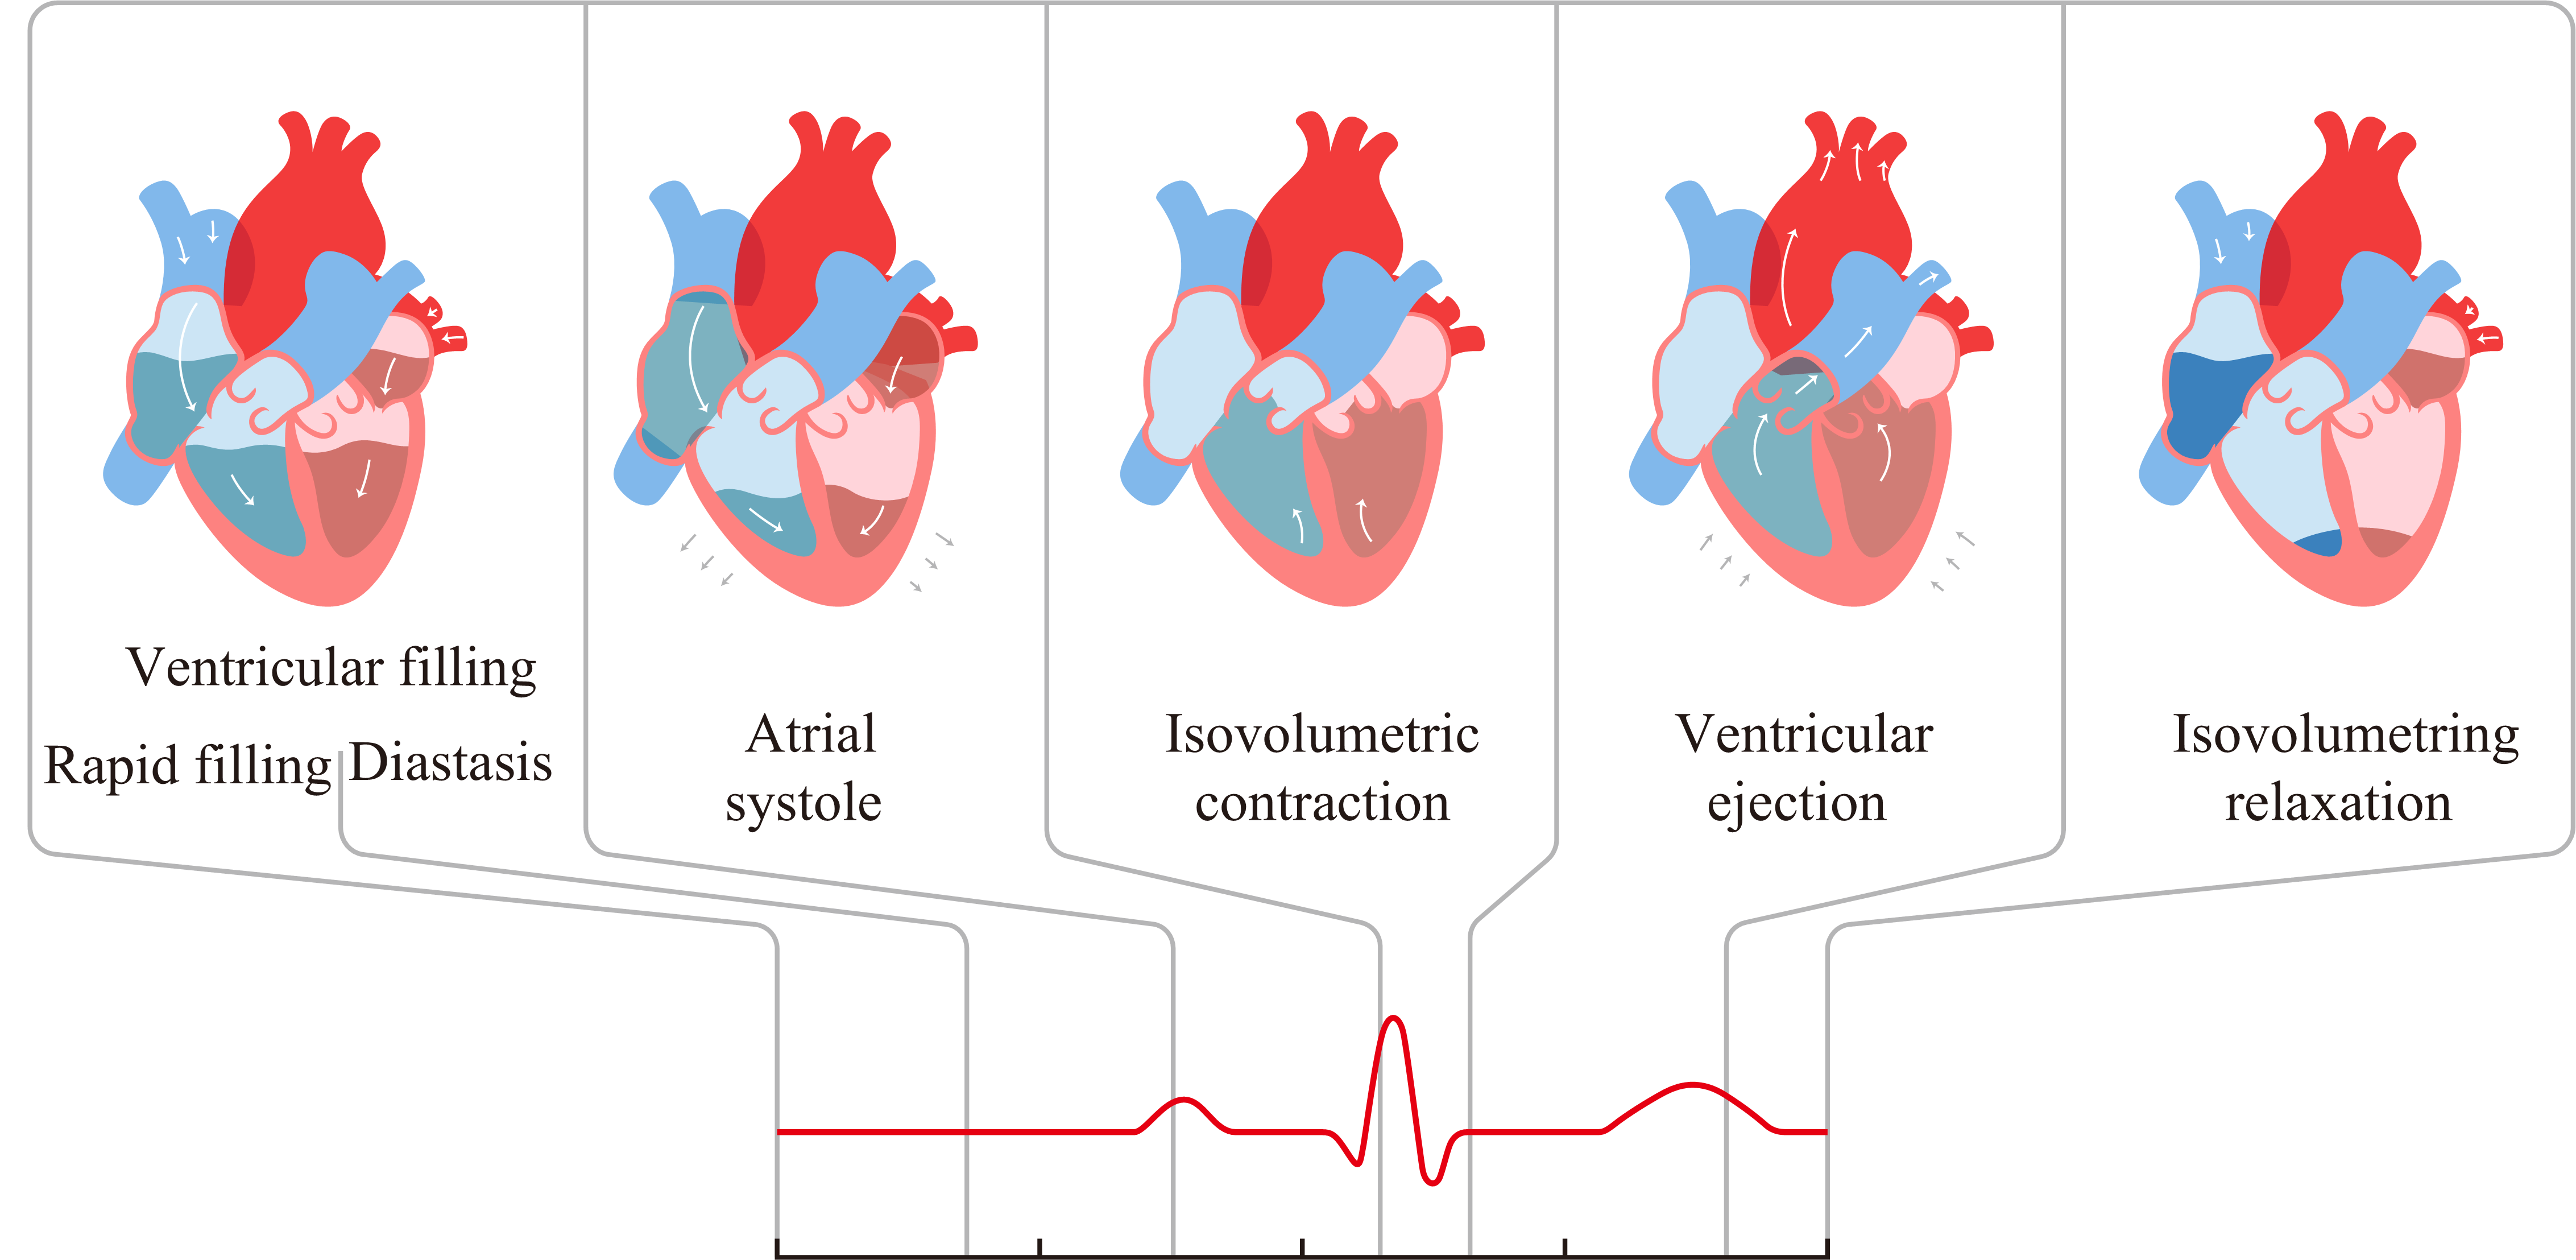
\includegraphics[width=9.5cm]{Figure/cycle}
    \caption{ (a) Schematic diagram of GCC signal transmission: the diagram illustrates the transmission of the signal from the transmitting electrodes in the RA to the receiving electrodes in the LV. (b) The Thevenin equivalent circuit on the myocardial tissue side. Circuit diagram of the impedance-matching network.}
    \label{fig:1}
\end{figure}

Effective multi-chamber pacing, essential for restoring physiological cardiac function, particularly under diverse pathological states that engender idiosyncratic CIC characteristics, is contingent upon a robust wireless communication system for precise inter-device synchronization. However, conventional wireless modalities present enduring limitations for this application: radio-frequency (RF) communication typically incurs prohibitive power consumption \cite{bose2018rf}; magnetic inductive coupling demands stringent device alignment \cite{li2018200mb, Islam2021Performance}; and ultrasonic methods suffer from inherent directivity constraints \cite{seyedi2013survey}. These intrinsic drawbacks severely curtail their suitability for the stable, ultra-low-power, and miniaturized communication rigorously demanded by multi-chamber LCPs.

In light of these challenges, conductive intra-cardiac communication (CIC), which leverages physiological tissue as the transmission medium, has emerged as a compelling paradigm, offering distinct potential in power efficiency and structural simplicity for LCP inter-device communication \cite{wu2020equivalent, opie2004heart, Khaleghi2020ConductiveImpulse, Wegmueller2010Signal, Teshome2016Galvanically}. Extensive research has focused on characterizing the CIC channel. Early investigations predominantly relied on static or quasi-static models, employing finite element analysis, numerical simulations, and \textit{in vivo} animal studies to delineate fundamental transmission properties \cite{bereuter2019leadless_sync, bereuter2018fundamental, Khaleghi2021Conductive_numerical, Maldari2020Frequency}. More recently, the dynamic nature of the CIC has begun to attract attention; for instance, the work of \cite{LiChen2023Investigation} provided valuable insights into general cardiac cycle dynamics via an \textit{ex vivo} platform, while our prior work contributed a time-varying equivalent circuit model for the CIC \cite{zilaingwei2024Time_varing_model_placeholder}.

While these foundational studies are crucial, a significant scientific gap persists: the vast majority of existing CIC transceiver designs are still predicated on oversimplified static or averaged channel models. This simplification, though facilitating initial analysis, fundamentally compromises the robustness and reliability of the resultant systems in authentic, dynamic physiological environments, as it fails to capture the intrinsically volatile nature of the intra-cardiac milieu. The rhythmic cardiac cycle itself (Fig.~\ref{fig:1}) engenders substantial and continuous channel gain fluctuations due to complex myocardial mechanics and hemodynamic shifts \cite{Zhang2019_placeholder_if_exists}. However, the channel dynamics under normal sinus rhythm can be considered relatively predictable compared to those encountered under specific pathological conditions, such as the arrhythmogenic profiles illustrated in Fig.~\ref{fig:0}. These conditions, characterized by irregular cardiac motion and adaptive physiological responses, often induce far more complex, erratic, and severe channel volatility. Regrettably, this critical layer of complexity—the profound and distinct impact of specific arrhythmogenic conditions on CIC dynamics—has been largely unaddressed in prior transceiver development, rendering existing systems potentially incapable of ensuring reliable communication when faced with these challenging real-world clinical scenarios \cite{Ryser2022ModulationScheme, Bereuter2019LeadlessResync}.

Given the stringent constraints on power and complexity in LCPs, the Super-Regenerative Receiver (SRR) architecture emerges as one of the most promising candidates, by virtue of its inherent simplicity and potential for achieving high sensitivity at very low power. A principal limitation of this architecture, however, is its acute sensitivity to variations in input signal amplitude (detailed in Section~\ref{subsec:srr_input_ber}). While this characteristic can be exploited for high gain under stable channel conditions, it transforms into a critical liability in the dynamic CIC environment, necessitating a sophisticated compensatory mechanism to unlock the SRR's full potential for reliable LCP communication.

To surmount this challenge, Automatic Gain Control (AGC) is indispensable. Traditional fully analog AGC systems, while offering rapid response, often utilize analog variable gain amplifiers (VGAs) with suboptimal linearity and imprecise gain control, and their fixed-threshold operation limits adaptability. Conversely, fully digital AGCs can achieve high precision and flexibility but typically at the expense of significant computational overhead and power consumption, incompatible with an LCP's stringent budget. Therefore, a critical technological need exists for an AGC solution that optimally synergizes rapid response, precise control, and extreme power efficiency.

In response to this imperative, this paper introduces a novel SRR system integrated with a meticulously co-designed hybrid analog-digital AGC mechanism. This architecture strategically leverages the rapid response of analog front-ends with the intelligent, fine-grained control afforded by digital processing, aiming to achieve robust compensation for dynamic CIC path gain variations while rigorously adhering to LCP power constraints. \textbf{This study, for the first time to our knowledge, systematically incorporates the complex and distinct CIC dynamic characteristics induced by specific arrhythmogenic pacemaker indications (such as AV block, as exemplified in Fig.~\ref{fig:av_block_types_placeholder_label}) into the design, optimization, and experimental validation of an SRR-based AGC system.} By adaptively stabilizing the signal level at the SRR input, our proposed system aims to markedly enhance Bit Error Rate (BER) performance and overall communication robustness, particularly under these challenging pathological conditions. The efficacy of this approach is demonstrated through \textit{ex vivo} experiments on a porcine heart platform, simulating channel conditions pertinent to the targeted pacing indications. These experiments reveal consistent receiver output and significantly improved BER performance despite substantial input signal fluctuations. This research not only presents a robust technological solution for a pressing clinical need in LCPs but also pioneers a design methodology for adaptive transceivers in highly dynamic biological environments, potentially paving the way for next-generation intelligent implantable devices with enhanced resilience and broader clinical applicability.



\begin{figure}[htbp]
    \centering
    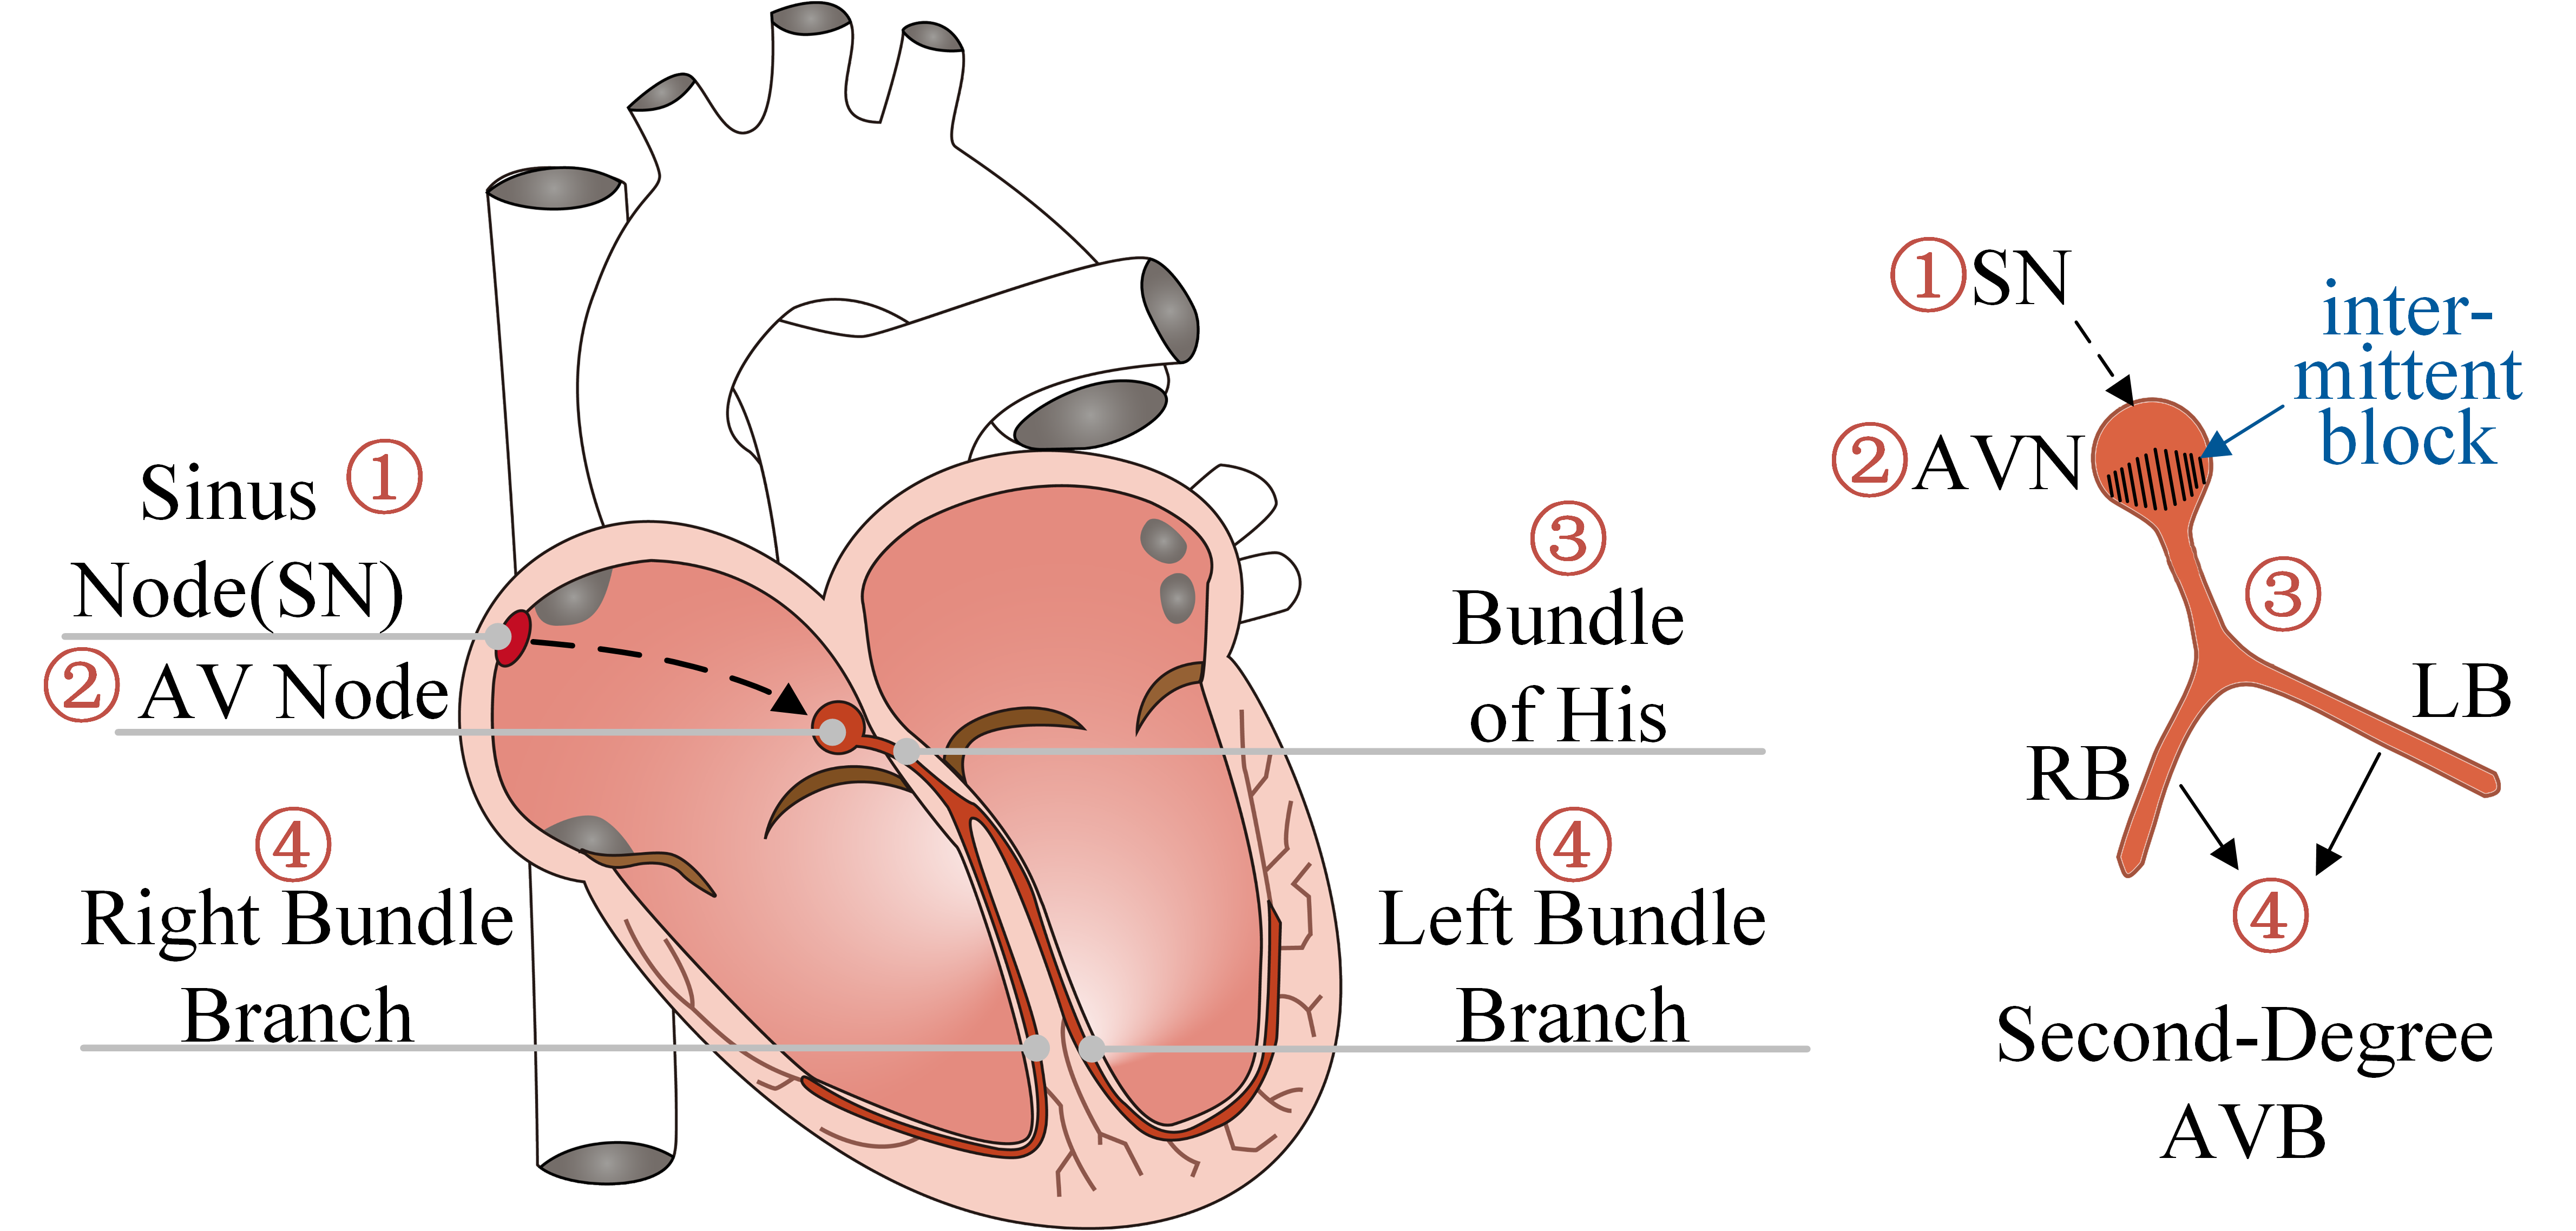
\includegraphics[width=8.3cm]{Figure/AVB}
    \caption{Schematic diagram of the cardiac conduction system and Second-degree Type I AVB.}
    \label{fig:0}
\end{figure}



\section{Methods}\label{sec:Methods}
\subsection{Dynamic Channel Characteristics and Impact on Receiver Performance}
\label{subsec:channel_and_impact}
Effective intra-cardiac communication (CIC) for multi-chamber leadless pacemakers is fundamentally challenged by the dynamic nature of the physiological environment. The rhythmic mechanical activities of the heart, encompassing myocardial contraction and relaxation, as well as variations in chamber volume and blood flow, collectively induce significant time-varying behavior in the CIC channel gain, denoted $G_c(t)$ \cite{your_ref_to_channel_dynamics}. While channel dynamics under normal sinus rhythm can be considered relatively predictable, the challenge is profoundly exacerbated under specific pathological conditions that constitute key pacemaker indications.  Arrhythmogenic profiles such as Atrioventricular Block (AVB), characterized by irregular cardiac motion and adaptive physiological responses, induce far more complex, erratic, and severe channel fluctuations compared to a healthy heart. This distinction is a central focus of this work and poses a formidable challenge to maintaining reliable wireless communication.

The Super-Regenerative Receiver (SRR) architecture, while attractive for its high sensitivity and low power consumption, exhibits an acute dependence on the stability of its input signal amplitude, $A_{in}(t)$ \cite{your_ref_to_srr_sensitivity}. In a typical front-end configuration without adaptive gain control, $A_{in}(t)$ is directly modulated by the channel gain:
\begin{equation}
    A_{in}(t) = G_{LNA} \cdot G_c(t) \cdot A_{tx}
    \label{eq:Ain_t_revised}
\end{equation}
where $G_{LNA}$ is the gain of a preceding Low Noise Amplifier and $A_{tx}$ is the transmitted signal amplitude. As a direct consequence of the fluctuating $G_c(t)$, $A_{in}(t)$ experiences substantial variations synchronous with the cardiac cycle.

This instability at the receiver input critically degrades demodulation performance. The discriminative capability of an SRR, quantified by the effective signal-to-noise ratio at its decision point, $SNR_{eff}(t)$, is proportional to the square of the input signal amplitude:
\begin{equation}
    SNR_{eff}(t) = \kappa \frac{A_{in}(t)^2}{N_{eff}}
    \label{eq:snr_eff_revised}
\end{equation}
where $\kappa$ is a proportionality constant encompassing circuit characteristics and $N_{eff}$ is the system's internal equivalent noise level. This quadratic relationship implies that even moderate fluctuations in $A_{in}(t)$ are amplified into severe variations in $SNR_{eff}(t)$.

For On-Off Keying (OOK) modulation, under the assumption of an Additive White Gaussian Noise (AWGN) channel, the instantaneous Bit Error Rate (BER), $P_e(t)$, can be expressed as a function of $SNR_{eff}(t)$:
\begin{equation}
    P_e(t) = \frac{1}{2}\text{erfc}\left(\sqrt{\frac{SNR_{eff}(t)}{2}}\right)
    \label{eq:Pe_t_revised}
\end{equation}

The consequences of this dependency chain are severe, particularly under the dynamic channel conditions induced by cardiac motion. During deep channel fades, the sharp decrease in $G_c(t)$ and, consequently, $A_{in}(t)$ leads to a collapse of the $SNR_{eff}(t)$. This results in a BER approaching 0.5, signifying a temporary but total failure of the communication link. Furthermore, the erratic and substantial signal fluctuations characteristic of arrhythmogenic states cause the instantaneous BER to vary wildly, with transient periods of high error rates disproportionately degrading the overall link reliability.

Compounding this primary challenge, the unstable input amplitude compromises the integrity of the decision-making process itself. The internal signal features leveraged by the SRR for demodulation, such as the oscillation envelope peak, become highly variable. This variability renders any fixed decision threshold, $V_{th}$, inherently suboptimal, leading to a further increase in bit errors. This confluence of SNR degradation and suboptimal thresholding robustly substantiates the necessity for an adaptive control system.

\subsection{Adaptive Receiver Architecture with Hybrid Gain Control}
\label{subsec:adaptive_architecture}

To counteract the severe performance degradation caused by dynamic channel fluctuations, we propose an adaptive receiver architecture incorporating a hybrid analog-digital Automatic Gain Control (AGC) system. This approach is designed to stabilize the signal amplitude at the input of the SRR core, thereby ensuring robust demodulation regardless of channel conditions. The architecture, depicted schematically in Figure~\ref{fig:framework}, is a closed-loop feedback system engineered for the stringent power and complexity constraints of LCPs.


\begin{figure}[!t]
    \centering
    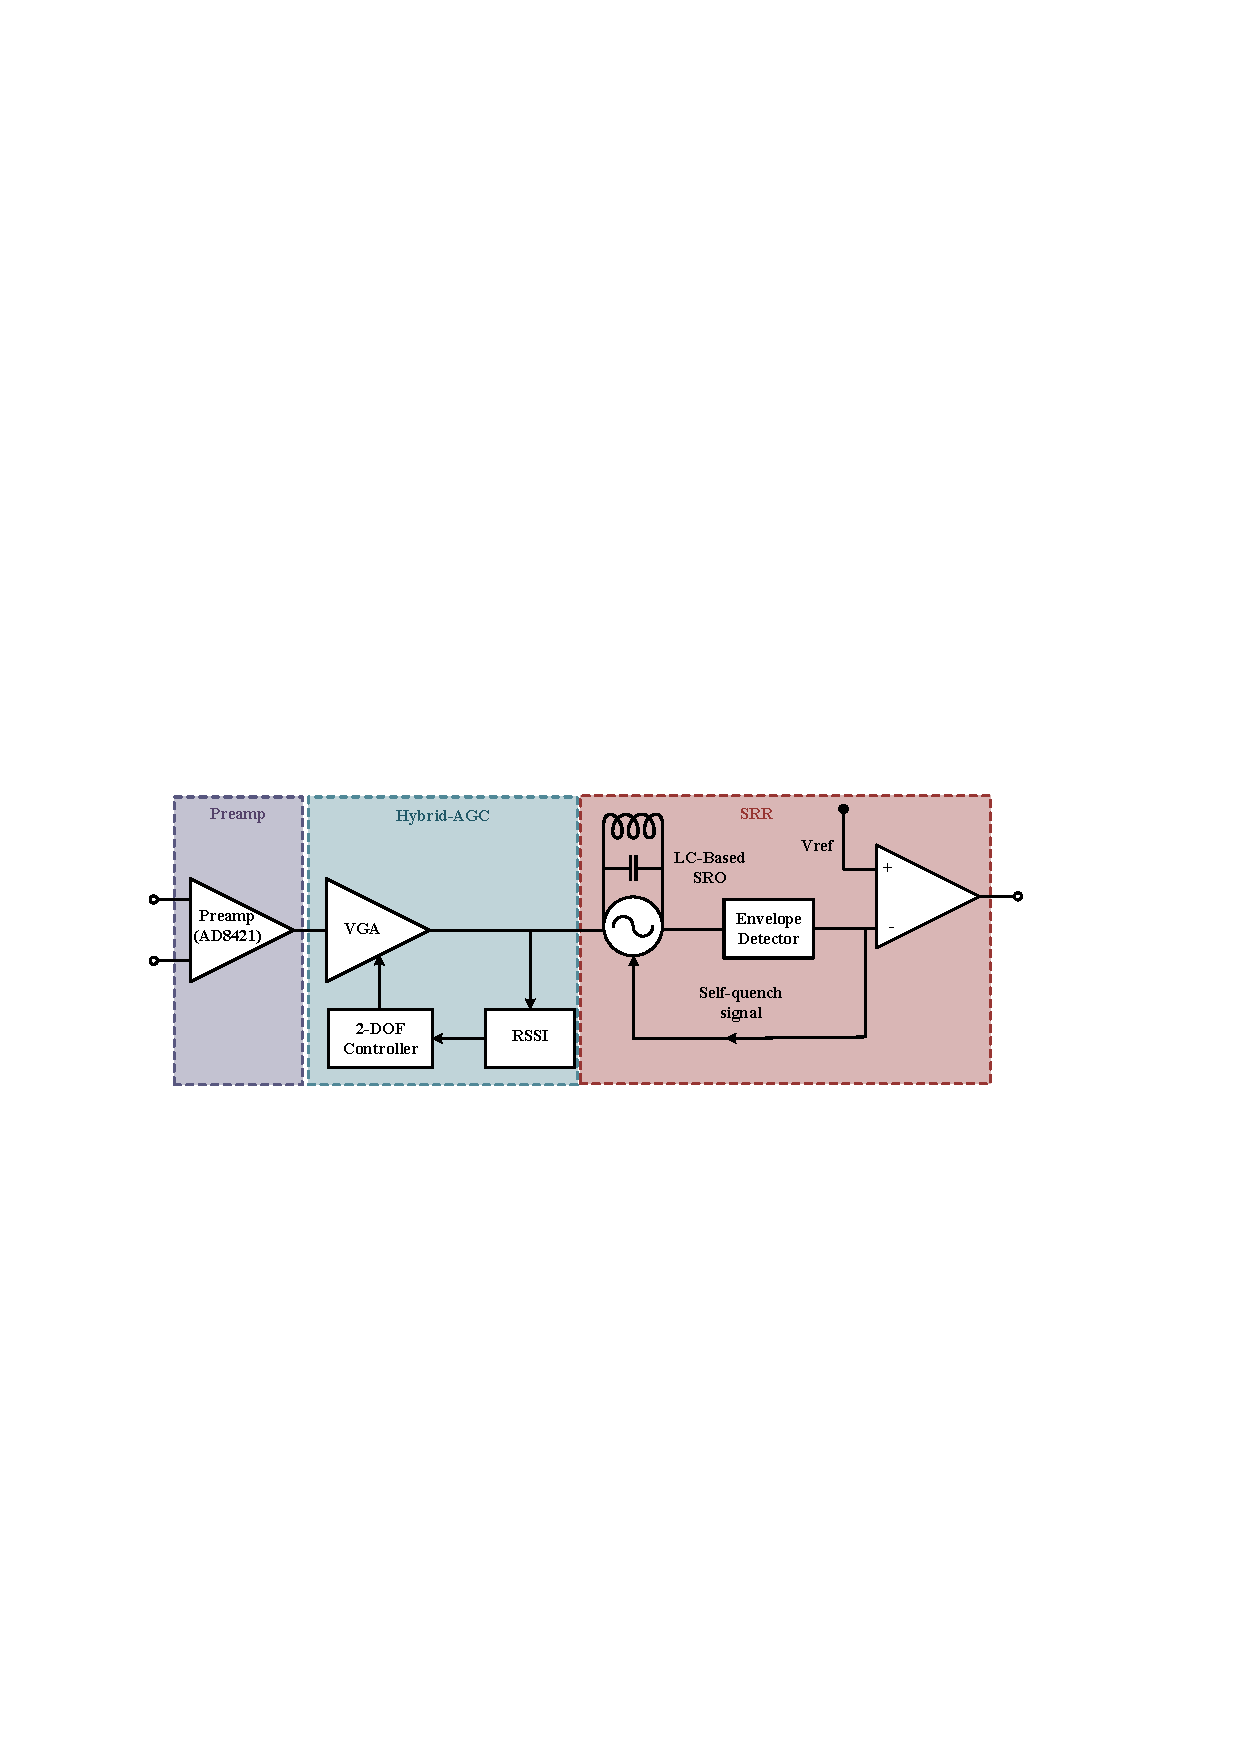
\includegraphics[width=8.3cm]{Figure/framework}
    \caption{Schematic of the transmitter used in the experiment. }
    \label{fig:framework}
\end{figure}


Incoming RF signals from the CIC are first processed by a Low Noise Amplifier (LNA) to minimize noise figure degradation. The amplified signal is then routed to a Variable Gain Amplifier (VGA), which serves as the primary gain control element. The VGA's gain, $G_{VGA}$, is dynamically modulated by an analog control voltage, $V_c$. The output of the VGA, $A_{in,AGC}(t)$, constitutes the stabilized input to the SRR core. The feedback path is initiated by a Received Signal Strength Indicator (RSSI) module, which measures the amplitude of the SRR's output envelope and generates a corresponding DC voltage, $V_{RSSI}$. This voltage is subsequently digitized by an Analog-to-Digital Converter (ADC), yielding a discrete-time signal, $A_{in,detected}(k)$, that represents the current signal level at the SRR input.

This hybrid architecture strategically leverages the distinct advantages of both analog and digital domains. The analog front-end (LNA, VGA, RSSI) provides a rapid response to signal level changes, while the digital back-end offers precise, flexible, and robust control. This synergy overcomes the limitations of traditional fully analog AGCs, which often suffer from suboptimal linearity and limited adaptability \cite{Zhao2023AnAF}, and fully digital AGCs, which can incur prohibitive power and computational overhead for this application \cite{Li2020DigitalAC}.



\subsection{Gain Compensation Principle and PID Control Algorithm}
\label{subsec:principle_and_algorithm}

The fundamental principle of the proposed AGC system is to dynamically adjust the VGA gain, $G_{VGA}$, to counteract the channel gain variations, $G_c(t)$, thereby maintaining a constant signal amplitude, $V_{target}$, at the SRR input. When the AGC loop achieves a stable or quasi-stable state, the relationship between the required $G_{VGA}$ and the instantaneous $G_c(t)$ can be derived from the overall system gain expression $A_{in,AGC}(t) = G_{VGA}(V_c,t) \cdot G_{LNA} \cdot G_c(t) \cdot A_{tx}$. By setting $A_{in,AGC}(t) \approx V_{target}$, the requisite VGA gain is:
\begin{equation}
    G_{VGA}(t) \approx \frac{V_{target}}{G_{LNA} \cdot G_c(t) \cdot A_{tx}}
    \label{eq:GVGA_compensation}
\end{equation}
Equation~\eqref{eq:GVGA_compensation} lucidly illustrates that the AGC system must modulate $G_{VGA}(t)$ to be approximately inversely proportional to the instantaneous channel gain. This self-regulating action is orchestrated by a Proportional-Integral-Derivative (PID) controller implemented in the digital domain.
The PID controller forms the intelligent core... An incremental PID formulation is employed... The controller calculates a control effort increment, $\Delta u_k$. This is derived from the standard discrete-time representation of a PID controller:
\begin{equation}
    \Delta u_k = K_p (e_k - e_{k-1}) + K_i T_s e_k + \frac{K_d}{T_s} (e_k - 2e_{k-1} + e_{k-2})
    \label{eq:PID_standard_discrete}
\end{equation}
where $K_p, K_i, K_d$ are the proportional, integral, and derivative gains, and $T_s$ is the sampling period. For efficient implementation, this equation is rearranged by grouping terms based on the error samples:
\begin{equation}
    \Delta u_k = (K_p + K_i T_s + \frac{K_d}{T_s}) e_k - (K_p + \frac{2K_d}{T_s}) e_{k-1} + (\frac{K_d}{T_s}) e_{k-2}
    \label{eq:PID_rearranged}
\end{equation}
This can be expressed in a more direct computational form:
\begin{equation}
    \Delta u_k = k_1 e_k - k_2 e_{k-1} + k_3 e_{k-2}
    \label{eq:PID_computational_form}
\end{equation}
where the coefficients $k_1 = K_p + K_i T_s + K_d/T_s$, $k_2 = K_p + 2K_d/T_s$, and $k_3 = K_d/T_s$ are pre-calculated to optimize the real-time control loop. The cumulative digital control output, $u_k = u_{k-1} + \Delta u_k$, is then converted by the DAC... The detailed iterative process is presented in Algorithm~\ref{alg:pid_control}.

The choice of a PID controller, as opposed to simpler control schemes, is a deliberate design decision to handle the complex dynamics of the CIC. The integral term is essential for annulling steady-state errors, ensuring the long-term average of the SRR input matches the target. The derivative term provides an anticipatory response to rapid changes in the channel gain, which is crucial for minimizing transient errors during the abrupt hemodynamic shifts characteristic of arrhythmogenic events. This sophisticated control is paramount for ensuring dependable communication in LCPs under challenging physiological conditions.



\begin{algorithm}[H]
    \caption{SRR Input Stabilization Algorithm}
    \label{alg:pid_control}
    \begin{algorithmic}[1] % The [1] enables line numbering
        \Require
            $V_{\text{target,dig}}$, $k_1, k_2, k_3$, $u_{\text{min\_dig}}, u_{\text{max\_dig}}$
        \Ensure
            $V_c(k)$

        \State Initialize $u_{\text{prev}}$; $e_{\text{prev1}} \gets 0$; $e_{\text{prev2}} \gets 0$
        \While{system is operating}
            \State $A_{\text{in,detected}}(k) \gets \text{Sample And Digitize SRR Input}()$
            \State $e_k \gets V_{\text{target,dig}} - A_{\text{in,detected}}(k)$
            \State $\Delta u_k \gets k_1 e_k - k_2 e_{\text{prev1}} + k_3 e_{\text{prev2}}$
            \State $u_k \gets u_{\text{prev}} + \Delta u_k$
            \State $u_k \gets \text{saturate}(u_k, u_{\text{min\_dig}}, u_{\text{max\_dig}})$

%            \Comment{Apply output limits}
            \State $V_c(k) \gets \text{Digital To Analog Conversion}(u_k)$
            \State $\text{Set VGA Control Voltage}(V_c(k))$
            \State \hspace{-1.5em} $\triangleright$ Update historical values for next iteration %
            \State $e_{\text{prev2}} \gets e_{\text{prev1}}$
            \State $e_{\text{prev1}} \gets e_k$
            \State $u_{\text{prev}} \gets u_k$
        \EndWhile
    \end{algorithmic}
\end{algorithm}




\section{Experimental Methodology and Setup} % 更改标题以包含方法学


The performance of the proposed hybrid AGC super-regenerative receiver was rigorously evaluated on a sophisticated \textit{ex-vivo} porcine heart platform. This platform was specifically engineered to emulate the dynamic channel conditions characteristic of both normal and arrhythmogenic cardiac cycles. The comprehensive experimental setup is depicted schematically in Figure~\ref{fig:agc_test_schematic}.




\begin{figure}[!t]
    \centering
    
\includegraphics[width=0.9\columnwidth]{figure/measure_setup} % 使用您的第三张图 (IMG_4224.jpeg)
    \caption{Photograph of the assembled experimental testbed, showcasing the peristaltic pump system, the cannulated \textit{ex-vivo} porcine heart, the signal generation instrumentation, and the custom-developed receiver module.}
    \label{fig:agc_test_schematic}
\end{figure}




The cornerstone of this experimental paradigm was the \textit{ex-vivo} porcine heart perfusion system (Fig.~\ref{fig:agc_test_schematic}), which was instrumental in recreating the heart's mechanical pumping action and the resultant dynamic channel environment. Fresh porcine hearts, procured from a local abattoir and selected based on criteria ensuring structural and physiological similarity to human hearts (e.g., weight range of adult pigs 90 to 120 kg, cell turnover rate considerations~\cite{karacolak2012dielectric}), served as the biological medium. A physiologically relevant simulated blood, with its electrical conductivity precisely matched to that of native human blood at body temperature (37°C), was formulated using deionized water and sodium chloride. This formulation adhered to established methodologies~\cite{maldari2020wide, gabriel1996dielectric}, and its conductivity profile was verified against real blood across the operational frequency spectrum of 100kHz to 20MHz (as illustrated in Fig.~\ref{fig:blood_conductivity_match_agc}), thereby minimizing impedance variations attributable to temperature or medium discrepancies. The governing relationship for the conductivity of the NaCl solution is given by~\cite{gadani2012effect}:
\begin{equation}
\begin{aligned}
    \sigma_{\mathrm{NaCl}}(25,N) & =N[10.394-2.3776N+0.68258N^2\\
&-0.13538N^3+1.00086\times10^{-2}N^4]
\end{aligned}
\end{equation}
where $N$ represents the normality of the solution.



\begin{figure}[!t]
    \centering
    
\includegraphics[width=0.9\columnwidth]{figure/Nor_Vol} % 使用您的第三张图 (IMG_4224.jpeg)
    \caption{Dynamic mapping relationship between the electrocardiogram (ECG) and right-sided chamber volumes (RA and RV) under simulated Normal Sinus Rhythm (NSR). This volumetric profile served as the baseline model for a healthy heart and formed the basis for emulating pathological conditions.
.}
    \label{nor}
\end{figure}


\begin{figure}[!t]
    \centering
    
\includegraphics[width=0.9\columnwidth]{figure/AVB_Vol} % 使用您的第三张图 (IMG_4224.jpeg)
    \caption{Emulation of a pathological cardiac cycle corresponding to an Atrioventricular Block (AVB) indication. The mapping illustrates an instance of intermittent conduction failure, where an atrial contraction (P-wave) is not followed by a ventricular response (QRS complex), leading to a distinct and irregular hemodynamic profile.}
    \label{avb}
\end{figure}


The perfusion system itself was comprised of a host computer, which served as the central controller, communicating via an RS-232 serial interface with two dual-channel peristaltic pumps (Model: [填写您的蠕动泵型号, e.g., BL400H/2*YZ15III]). These pumps, through a network of silicone tubing securely cannulated to the heart's major vessels (e.g., superior vena cava for atrial inflow, aorta/pulmonary artery for ventricular outflow), precisely governed the flow of the simulated blood. Custom-developed serial control software (SSCOM V5.13) enabled the dynamic adjustment of pump speed and direction. This capability was leveraged to meticulously vary the intracardiac chamber volumes over time, thereby emulating the distinct hemodynamic phases of a normal cardiac cycle (isovolumetric relaxation, rapid filling, diastasis, atrial contraction, isovolumetric contraction, rapid ejection, and slow ejection~\cite{1998Heart}). The specific volumetric profiles for these phases (detailed in TABLE~\ref{tab:table1_agc}) were derived from comprehensive analyses of published human cardiac chamber volume data~\cite{2006Normalized,2006Reference,2013Reference,maceira2010reference} and motion patterns~\cite{chen2022investigation}, ensuring accurate reproduction of impedance characteristics. The dynamic mapping relationship between the ECG and the RA/LV volumes, which underpins this simulation, is depicted in Fig.~\ref{fig:ecg_volume_map_agc}. This controlled volumetric modulation was critical for simulating both NSR and the specific pathophysiological dynamics of Second-degree Type I AVB.

\begin{table}[!t] % 如果您有这个表格，可以保留并重命名label
\centering
\caption{Cardiac Cycle Phases and Corresponding Chamber Volumes Utilized for Dynamic Simulation}
\begin{tabular}{cccc}
\hline
\text{\bfseries Phase} & \text{\bfseries Duration(s)} & \text{\begin{tabular}[c]{@{}c@{}}\bfseries Left Cardiac\\\bfseries Volume (mL)\end{tabular}} & \text{\begin{tabular}[c]{@{}c@{}}\bfseries Right Cardiac\\ \bfseries Volume (mL)\end{tabular}} \\ \hline
\text{\begin{tabular}[c]{@{}c@{}}\bfseries Isovolumetric\\ \bfseries Relaxation\end{tabular}} & 0.07 & 120.00 & 150.00 \\
\text{\bfseries Rapid filling} & 0.11 & 173.44 & 202.88 \\
\text{\bfseries Diastasis} & 0.22 & 191.25 & 220.50 \\
\text{\begin{tabular}[c]{@{}c@{}}\bfseries Atrial\\\bfseries  Contraction\end{tabular}} & 0.10 & 215.00 & 244.00 \\
\text{\begin{tabular}[c]{@{}c@{}}\bfseries Isovolumetric\\\bfseries  Contraction\end{tabular}} & 0.05 & 215.00 & 244.00 \\
\text{\bfseries Rapid ejection} & 0.10 & 151.67 & 181.34 \\
\text{\bfseries Slow ejection} & 0.15 & 120.00 & 150.00 \\ \hline
\end{tabular}
\label{tab:table1_agc}
\end{table}

\begin{figure}[!t]
    \centering
    \includegraphics[width=0.95\columnwidth]{figure/Mea.BER} % 使用您的第二张图 (实验装置图.png)
    \caption{Schematic diagram of the comprehensive experimental setup for the evaluation of the hybrid AGC super-regenerative receiver. The configuration integrates a signal generator (SG), impedance-matching baluns, an \textit{ex-vivo} porcine heart subjected to controlled perfusion via peristaltic pumps to emulate dynamic intracardiac channel conditions, the super-regenerative receiver (SRR) incorporating the proposed AGC, and a data acquisition (DAQ) system interfaced with a host computer.}
    \label{??}
\end{figure}



The communication testbed was then integrated with this dynamic \textit{ex-vivo} heart model. A [填写您的信号发生器型号, e.g., Rigol DSG815] signal generator (SG) was employed to produce an On-Off Keying (OOK) modulated carrier signal at a designated intracardiac communication frequency of [填写您的CIC频率, e.g., 1 MHz]. The OOK signal, encoding a pseudo-random bit sequence (PRBS) for robust error rate analysis, was transmitted at an amplitude of [填写发射幅度, e.g., X mVpp]. Signal transmission into and reception from the cardiac tissue were facilitated by a pair of OptiSense™ 1999 active fixation pacemaker electrodes. One electrode was strategically implanted within the right atrium (RA) to function as the transmitter, while the second was placed in the right ventricle (RV) to serve as the receiver, thereby establishing the RA-RV intracardiac communication link under investigation. To ensure efficient signal coupling and to mitigate common-mode interference, wideband baluns (Model: [填写您的Balun型号, e.g., Mini-Circuits FTB-1-6*A15+]) were interfaced between the SG/receiver and the bipolar electrode pairs. The signal captured by the RV electrode, subsequent to passing through its respective balun, constituted the input to our custom-developed super-regenerative receiver incorporating the novel hybrid AGC (SRR-AGC).

Quantitative assessment of the SRR-AGC's performance involved several key measurements. The demodulated binary output stream from the receiver was captured by a data acquisition (DAQ) system [如果知道DAQ型号，可以写上, e.g., a National Instruments PCI-6115 card] connected to the host computer, which then computed the Bit Error Rate (BER) by comparing the received sequence against the known transmitted PRBS. This BER analysis was conducted across a range of data rates, from 500 bps to 5 kbps. Simultaneously, critical analog signals reflective of the AGC's internal operation – specifically, the VGA output amplitude (which represents the stabilized input to the SRR core) and the dynamically varying VGA control voltage (`Vg`) – were meticulously monitored and digitized using a digital storage oscilloscope (Model: [填写您的示波器型号, e.g., Rigol MSO5000 series]). The overarching experimental protocol entailed: first, establishing a stable, simulated cardiac condition (either NSR or Second-degree Type I AVB) within the \textit{ex-vivo} heart; second, initiating OOK signal transmission through the thus-formed dynamic RA-RV channel; and third, performing prolonged data acquisition to ensure statistically robust BER calculations (typically involving the transmission of $10^5$ to $10^6$ bits for each reported BER value). This entire sequence was systematically repeated for all specified data rates and cardiac states. For essential baseline comparisons, denoted as "Without AGC" trials, the AGC feedback loop within the SRR-AGC was intentionally disabled, and the VGA was operated at a fixed, predetermined gain. This fixed gain was chosen to [请在这里具体说明这个固定增益是如何选择的, e.g., "correspond to the optimal gain for the mean observed channel attenuation under NSR, providing a stringent comparative benchmark," or "represent a typical operational gain in the absence of dynamic compensation."]. [If applicable: "To ensure the statistical validity and account for inherent biological variability, these experimental procedures were replicated across multiple porcine heart preparations (N=3)."]






\section{Experimental Results}
\label{sec:results}

The performance of the proposed hybrid analog-digital Automatic Gain Control (AGC) system for Super-Regenerative Receiver (SRR)-based intracardiac communication was rigorously evaluated. The key findings are presented below, demonstrating the system's efficacy in mitigating dynamic channel variations, particularly under simulated pathological conditions such as Mobitz Type Atrioventricular Block (AVB).




\subsection{Dynamic Intracardiac Channel Characteristics}
Figure~\ref{fig:path_gain_variation} illustrates the inherent dynamic variations in the Right Atrial to Right Ventricular (RA-RV) intracardiac channel path gain, measured over several cardiac cycles using an \textit{ex-vivo} porcine heart platform. Under simulated healthy heart conditions (Fig.~\ref{fig:path_gain_variation}(a)), the path gain exhibits periodic fluctuations of approximately \SI{10}{\decibel} to \SI{15}{\decibel}, synchronous with the cardiac mechanical activity. These variations become more pronounced and potentially irregular under simulated Mobitz Type I AVB conditions (Fig.~\ref{fig:path_gain_variation}(b)), with peak-to-peak fluctuations reaching up to \SI{15}{\decibel} to \SI{20}{\decibel}. Data from three different heart preparations (Heart-A, Heart-B, Heart-C) show consistent dynamic patterns, albeit with inter-subject variability. These results underscore the significant challenge posed by channel volatility to reliable Leadless Pacemaker (LCP) communication, necessitating an effective compensation mechanism.


\begin{figure}[!t] % 使用 [H] 强制图片在当前位置 (需要 float 包)
    \centering
    % 假设您的图片文件名为 path_gain_variation.png/pdf/eps
    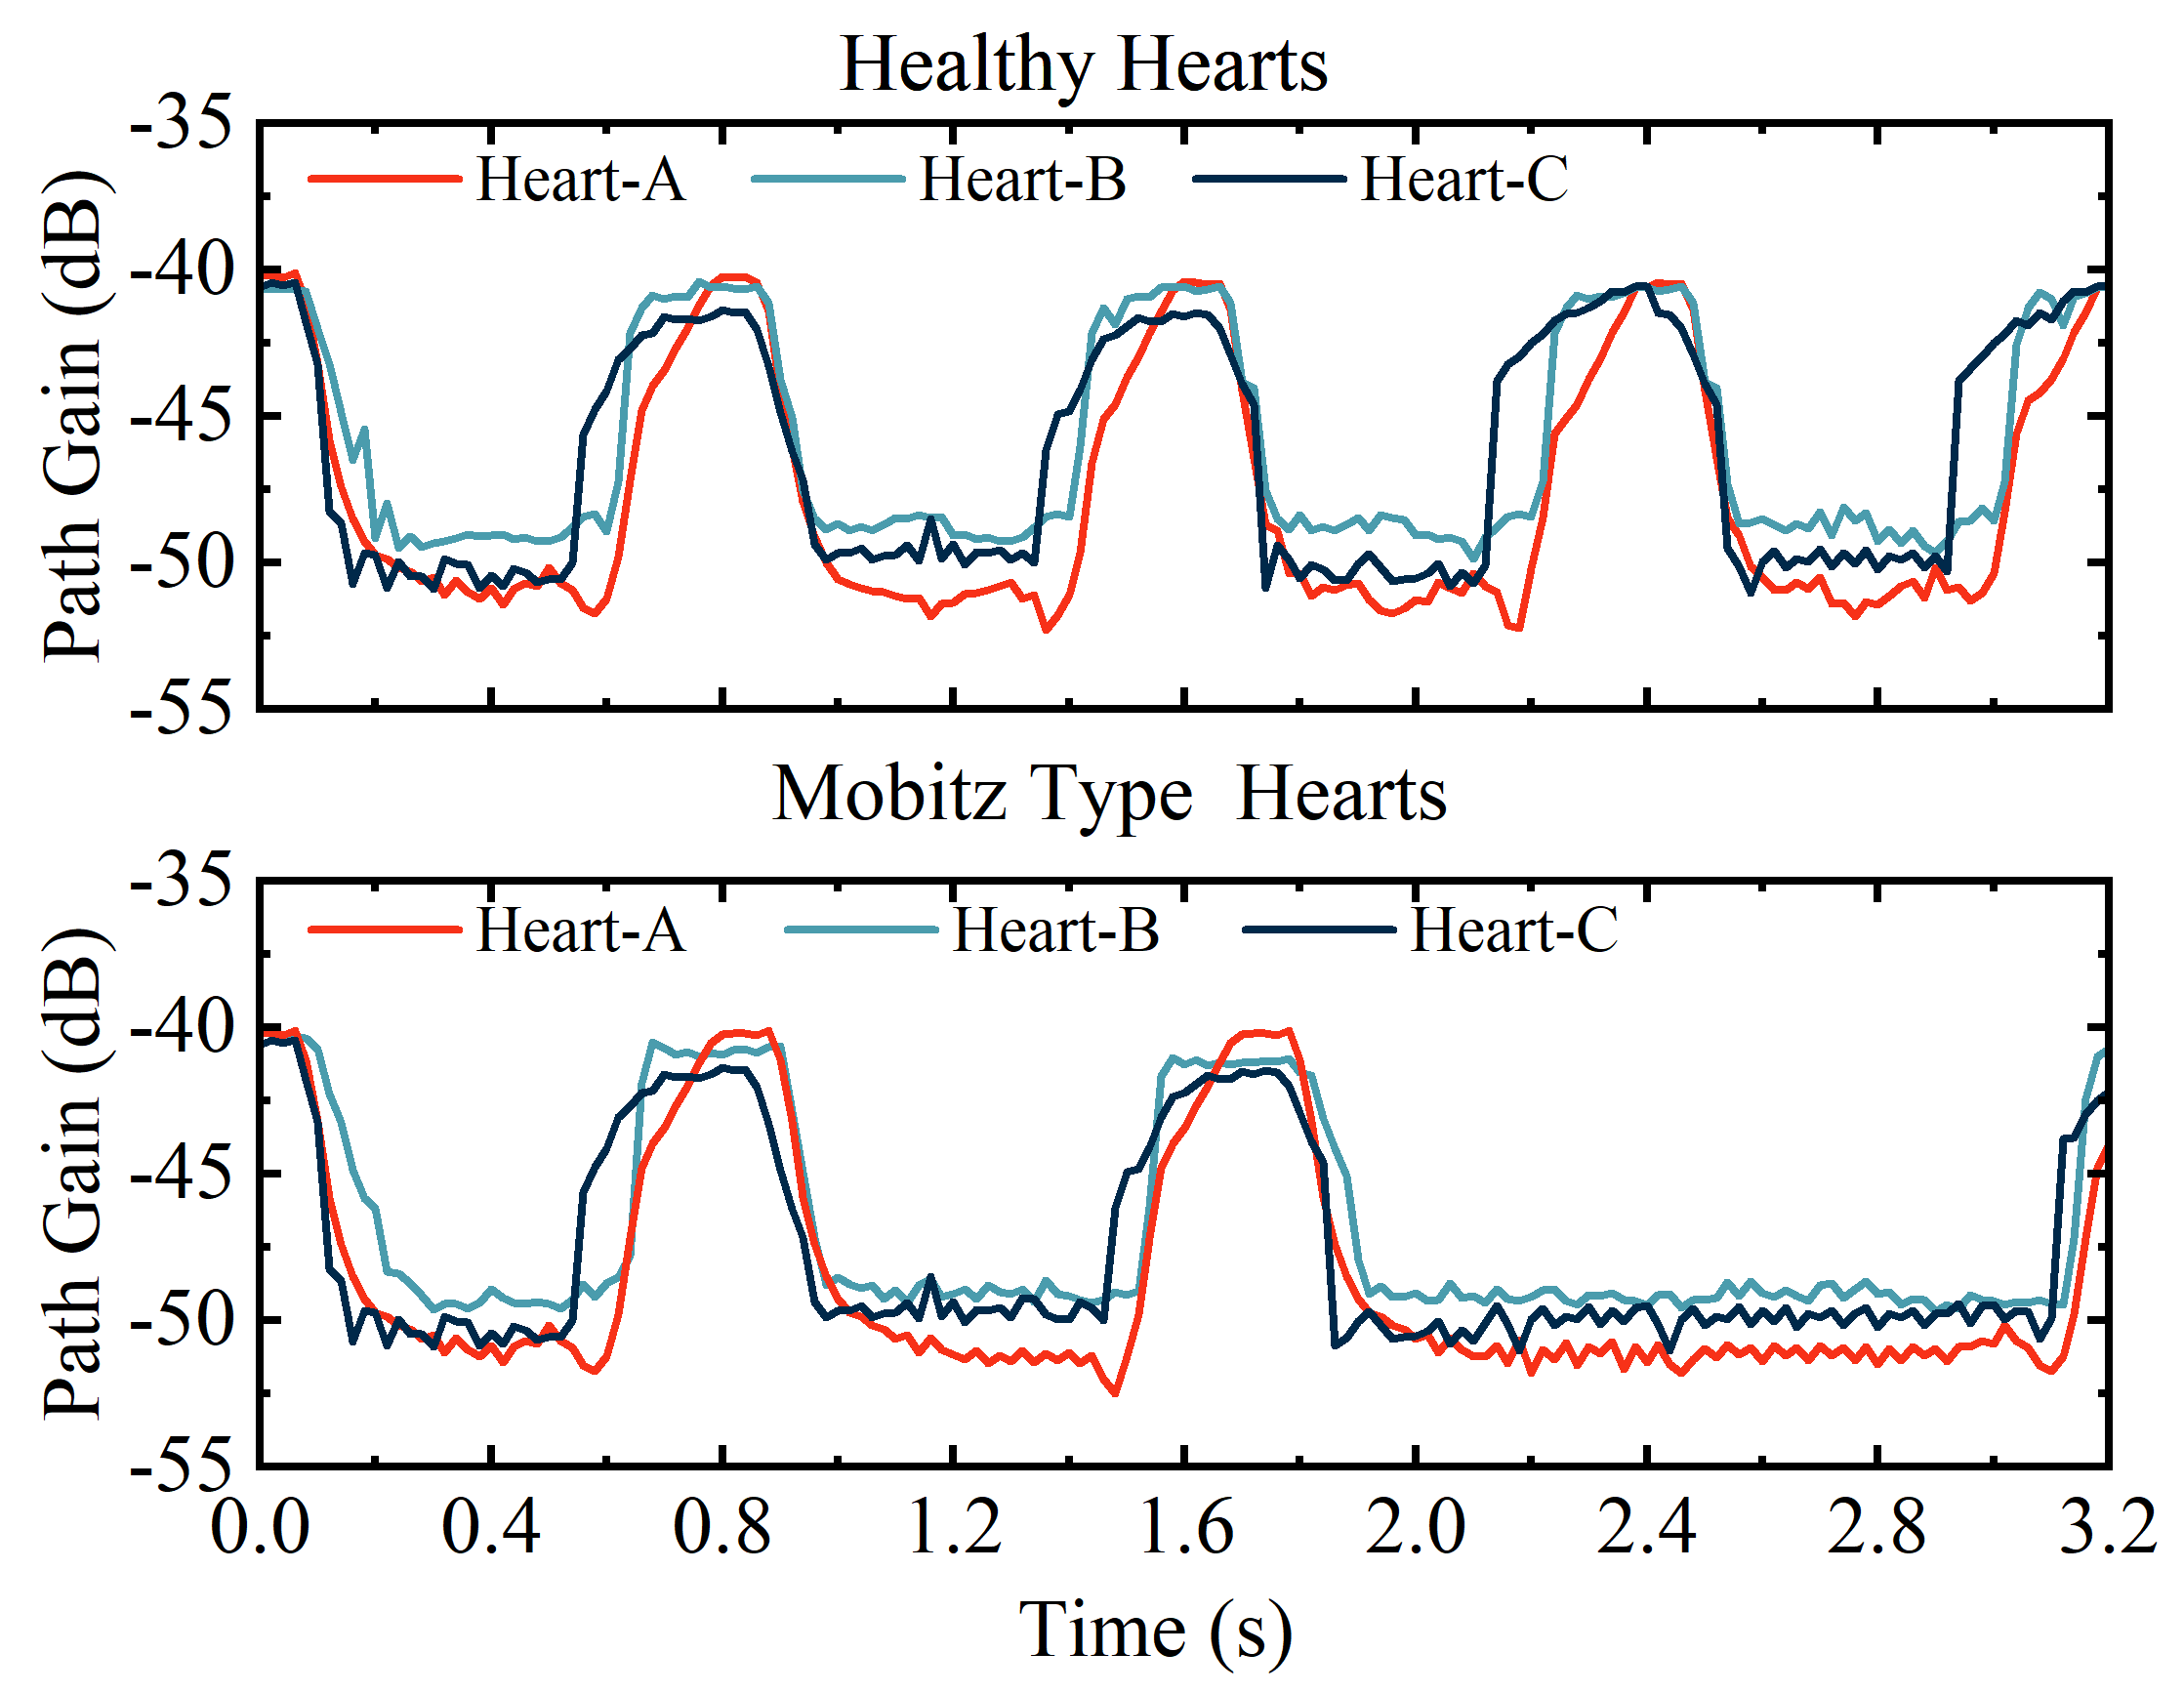
\includegraphics[width=0.9\linewidth]{Figure/signal_heart} % 替换为您的图片文件名
    \caption{Dynamic path gain variation of the RA-RV intracardiac channel. (a) Under simulated healthy heart conditions. (b) Under simulated Mobitz Type I AVB conditions. Results from three different ex-vivo porcine heart preparations (Heart-A, Heart-B, Heart-C) are shown.}
    \label{fig:path_gain_variation}
\end{figure}


\subsection{AGC System Performance in Signal Stabilization}
The effectiveness of the proposed hybrid AGC system in stabilizing the SRR input signal is demonstrated in Figure~\ref{fig:agc_stabilization}. The experiments were conducted under simulated Mobitz Type I AVB conditions, which induce severe channel dynamics. The reference Electrocardiogram (ECG) signal (Fig.~\ref{fig:agc_stabilization}(a)) provides a temporal marker for the cardiac cycle. Without AGC (Fig.~\ref{fig:agc_stabilization}(b)), the received signal amplitude at the SRR input (after the Low Noise Amplifier, LNA) fluctuated significantly from approximately \SI{1.5}{\milli\volt} to \SI{5.0}{\milli\volt}, directly reflecting the path gain variations observed in Fig.~\ref{fig:path_gain_variation}(b).

In contrast, when the hybrid AGC system was activated, the Proportional-Integral-Derivative (PID) controller dynamically adjusted the Variable Gain Amplifier (VGA) control voltage ($V_g$), as shown in Fig.~\ref{fig:agc_stabilization}(c). This control voltage, ranging from approximately \SI{12}{\milli\volt} to \SI{25}{\milli\volt}, exhibited an inverse relationship to the uncompensated signal amplitude, actively modulating the VGA gain to counteract channel losses or gains. Consequently, the SRR input signal amplitude was effectively stabilized around the target level of \SI{100}{\milli\volt} (Fig.~\ref{fig:agc_stabilization}(d)), with residual peak-to-peak fluctuations reduced to less than \SI{1}{\milli\volt} (i.e., approximately 1\%). This demonstrates the AGC's capability to provide a consistent signal level to the SRR despite substantial channel dynamics.

\begin{figure}[!t]
    \centering
    % 假设您的图片文件名为 agc_stabilization_effects.png/pdf/eps
    \includegraphics[width=0.9\linewidth]{Figure/Receiver_power} % 替换为您的图片文件名
    \caption{Effectiveness of the hybrid AGC system in stabilizing the receiver input signal under simulated Mobitz Type I AVB conditions. (a) Reference Electrocardiogram (ECG) signal. (b) Received signal amplitude at the SRR input without AGC. (c) Dynamic VGA control voltage ($V_g$) generated by the PID controller. (d) Received signal amplitude at the SRR input with the AGC activated, showing stabilization around the \SI{100}{\milli\volt} target.}
    \label{fig:agc_stabilization}
\end{figure}

\subsection{Impact of AGC on OOK Signal Demodulation}
The impact of the stabilized SRR input signal on the On-Off Keying (OOK) demodulation process is illustrated in Figure~\ref{fig:ook_demodulation}. Figure~\ref{fig:ook_demodulation}(a) shows the transmitted OOK baseband data sequence (0.5V logic high). The corresponding OOK modulated signal received at the SRR input, after being processed by the VGA with active AGC, is shown in Figure~\ref{fig:ook_demodulation}(b). Despite the underlying dynamic channel, the amplitude of the received OOK bursts is maintained at a relatively constant level (around \SI{0.3}{\volt} to \SI{0.4}{\volt} peak in this example, corresponding to the \SI{100}{\milli\volt} RMS target after LNA/VGA gain) due to the AGC action. As a result, the SRR was able to reliably demodulate the signal, producing a clean baseband output (Fig.~\ref{fig:ook_demodulation}(c)) that closely matches the transmitted sequence with correct logic levels. This qualitative result indicates successful data recovery under dynamic conditions facilitated by the AGC.

\begin{figure}[!t]
    \centering
    % 假设您的图片文件名为 ook_waveforms.png/pdf/eps
    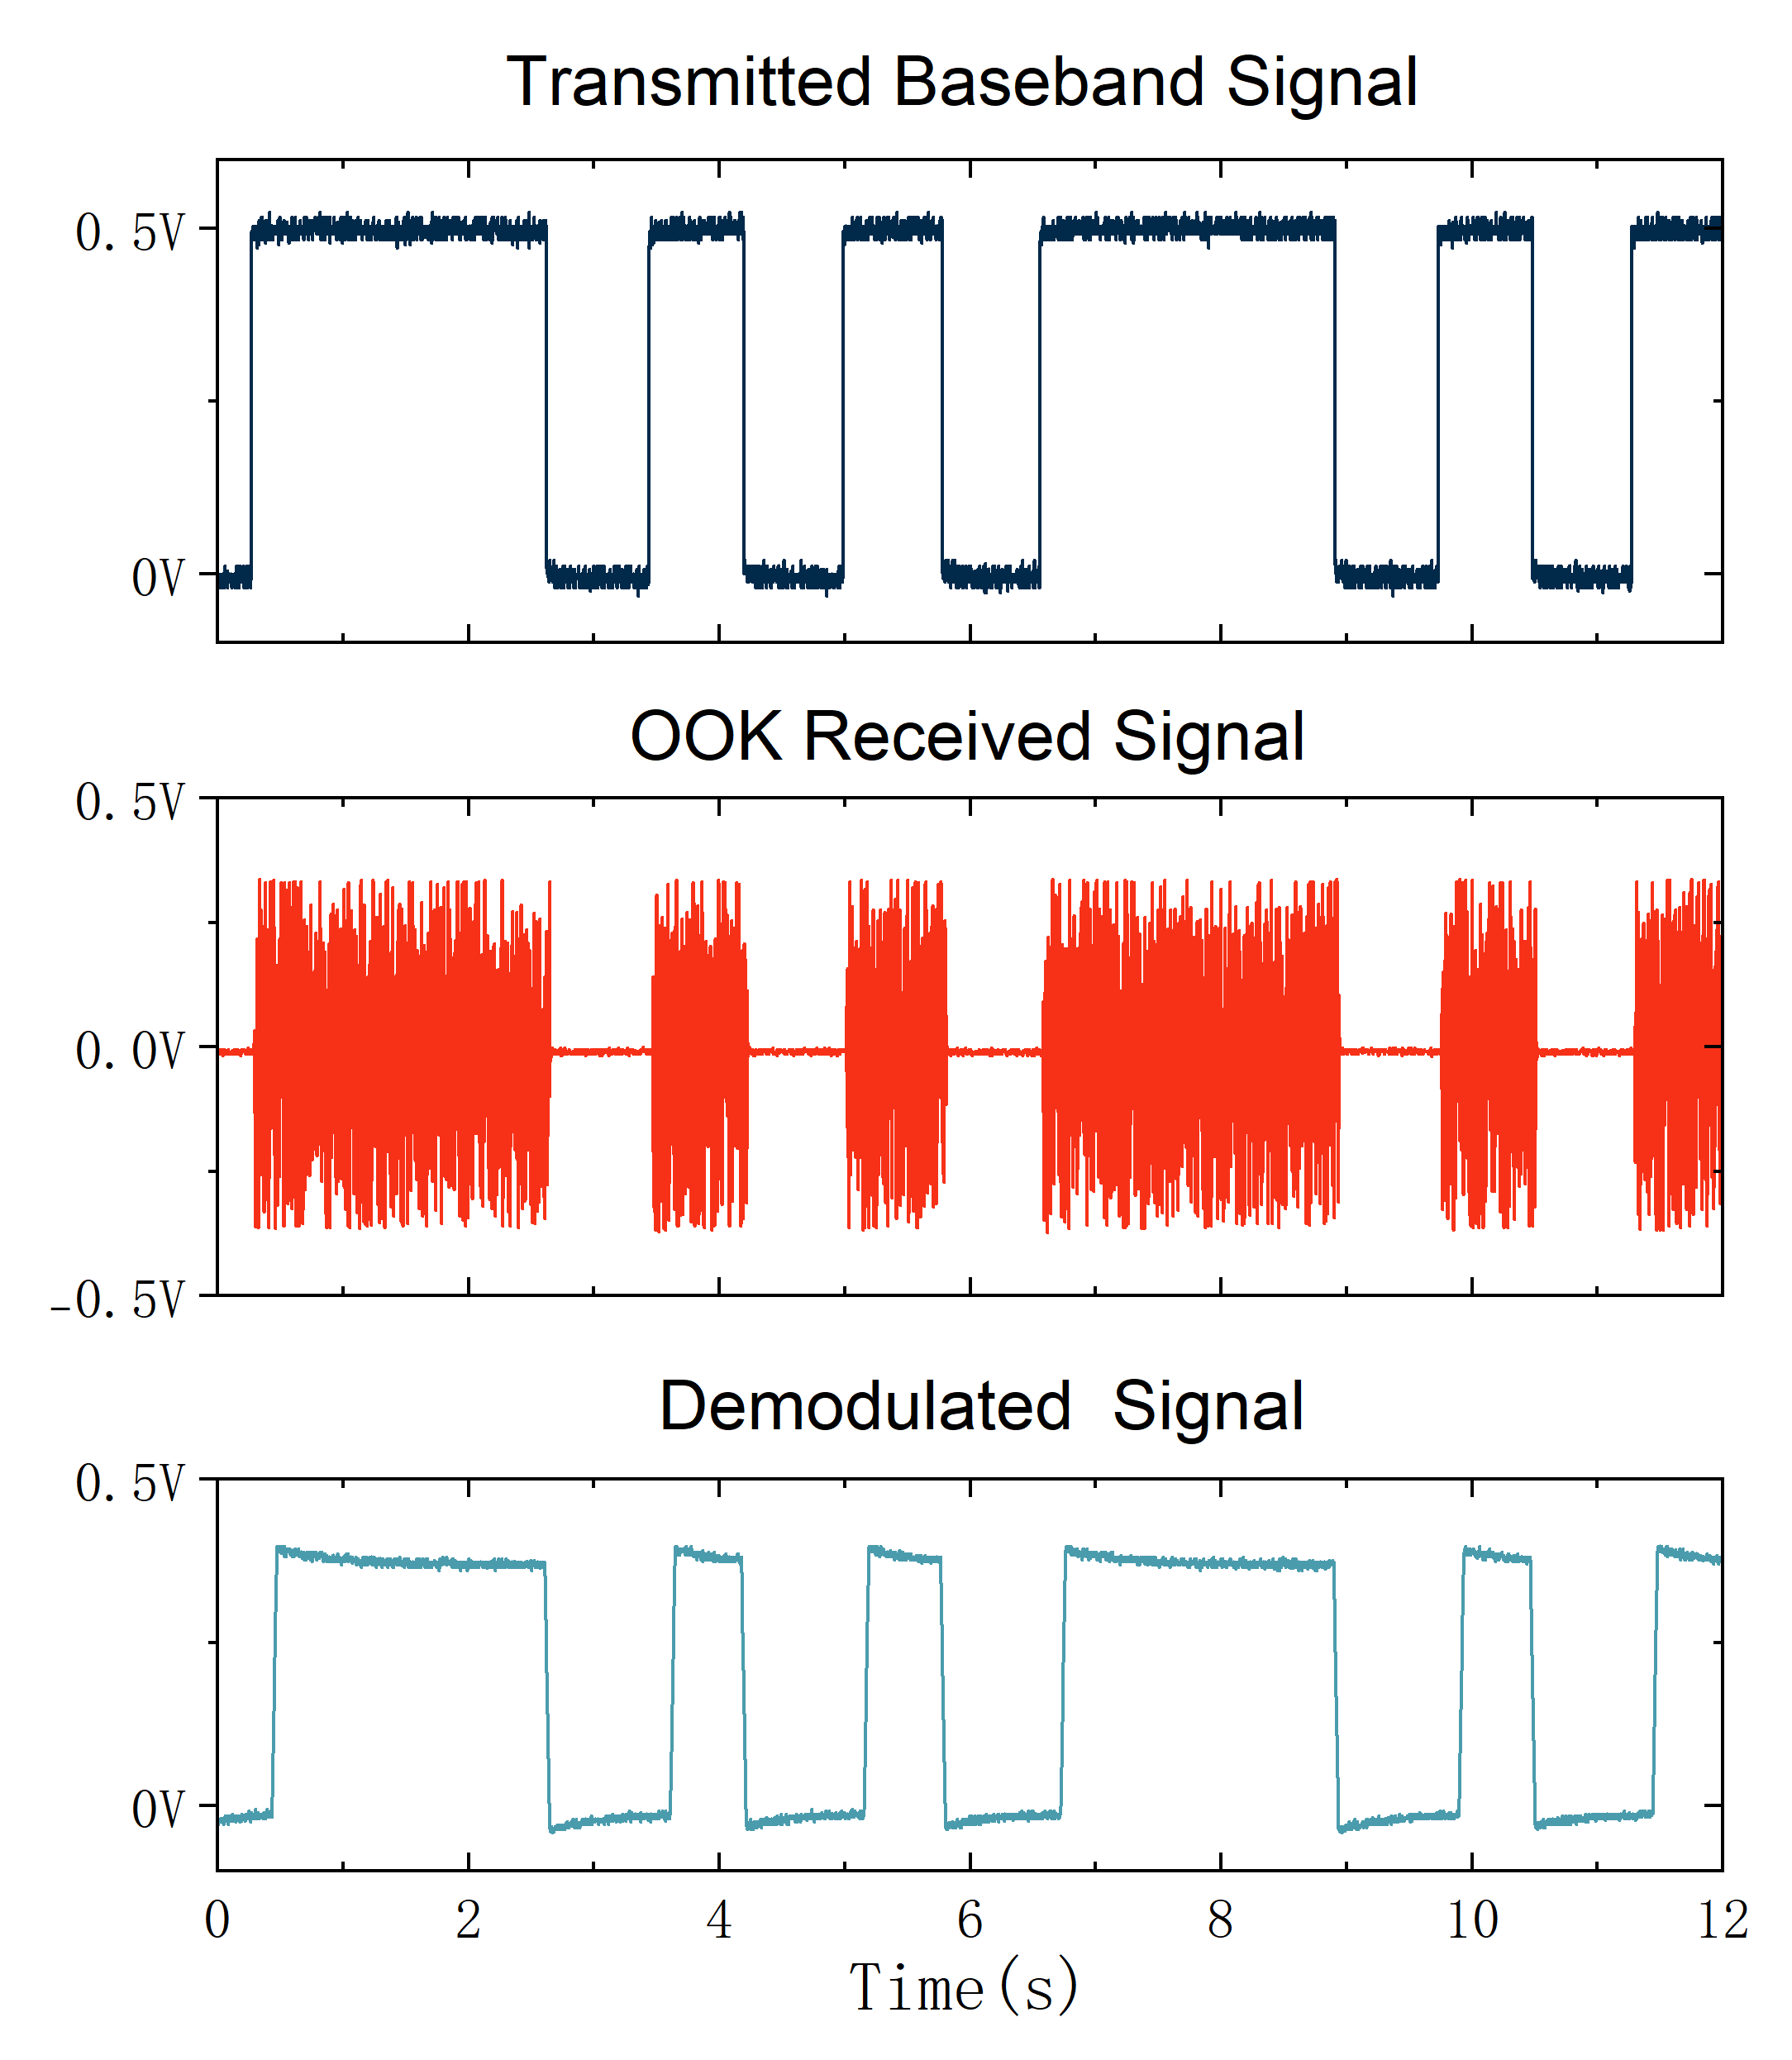
\includegraphics[width=0.8\linewidth]{Figure/ook} % 替换为您的图片文件名
    \caption{OOK signal waveforms at different stages of the communication system with AGC activated. (a) Transmitted baseband signal. (b) OOK received signal at the SRR input (after VGA with AGC). (c) Demodulated baseband signal at the SRR output.}
    \label{fig:ook_demodulation}
\end{figure}

\begin{figure}[!t]
    \centering
    % 假设您的图片文件名为 ber_vs_datarate.png/pdf/eps
    \includegraphics[width=0.8\linewidth]{Figure/BER} % 替换为您的图片文件名
    \caption{Bit Error Rate (BER) performance comparison with and without AGC across different data rates under simulated Mobitz Type I AVB conditions. The yellow line indicates the percentage improvement in BER achieved with AGC. Error bars represent standard deviation from $N=5$ independent trials.}
    \label{fig:ber_performance}
\end{figure}

\subsection{Bit Error Rate (BER) Improvement}
Quantitative assessment of the communication reliability was performed by measuring the Bit Error Rate (BER) with and without the AGC system across a range of data rates from \SI{500}{bps} to \SI{5}{kbps}, under simulated Mobitz Type I AVB channel conditions. As presented in Figure~\ref{fig:ber_performance}, the proposed AGC system significantly improved the BER performance. For instance, at a data rate of \SI{3}{kbps}, the BER was reduced from approximately \num{4.5e-4} (without AGC) to \num{9e-5} (with AGC). The percentage improvement in BER, calculated as (($\text{BER}_{\text{without\_AGC}} - \text{BER}_{\text{with\_AGC}}) / \text{BER}_{\text{without\_AGC}}) \times 100\%$, ranged from 54.8\% at \SI{500}{bps} to a substantial 83.7\% at \SI{5}{kbps}, as indicated by the yellow line and right y-axis. The error bars in Fig.~\ref{fig:ber_performance} represent the standard deviation from $N=5$ independent trials (replace $N=5$ with your actual number of trials), indicating the consistency of the observed improvements. These results quantitatively confirm that the dynamic path gain compensation provided by the AGC system translates directly into enhanced communication robustness.




\begin{table*}[htbp]\caption{POWER PERFORMANCE COMPARISON WITH PREVIOUS CONDUCTIVE INTRABODY COMMUNICATION PROTOTYPES}
    \label{table2}
    \begin{threeparttable}
 \begin{tabularx}{\textwidth}{XXXXXX}
\toprule

\bfseries Publication   & \bfseries L. Bereuter et al.~\cite{bereuter2019leadless} &\bfseries  Ryser et al.~\cite{ryser2022modulation}& \bfseries Khaleghi et al.~\cite{khaleghi2020conductive} & \bfseries Yuk et al.~\cite{yuk2020implantable}  &\bfseries This work\tnote{a}
 \\
\midrule
\bfseries Measurement Type & In-vivo                   & In-vitro           & In-vitro       & In-vivo / In-vitro     & In-vitro  \\
\bfseries Channel          & Porcine Heart             & Porcine Heart      & Porcine Heart  & Porcine Heart & Porcine Heart\\
\bfseries Frequency [MHz]       & 1                        & 1.5               & 0.01-10       &DC-20  & 10   \\
\bfseries TX Power[mW]\tnote{b}
       & $>$360           & 97                 & 0.025     &0.57     & 198        \\
\bfseries RX Power[mW]\tnote{b}
     & $>$465            & 152   & 230   &0.062         & 390      \\
\bfseries Technology       & Discrete                  & Discrete           & Discrete     &110nm CMOS  & Discrete      \\
\bottomrule
\end{tabularx}

 \begin{tablenotes}
        \footnotesize
        \item[a] The DDS is used for frequency adjustment, making it tunable.
        \item[b] Only analog power.

\end{tablenotes}

\end{threeparttable}
\end{table*}












\bibliographystyle{ieeetr}

\bibliography{Reference}

\end{document}


